% !TeX program = xelatex
\documentclass{scrartcl}

% This commad is defined in the makefile to generate the different
% language versions. If one compiles it directly this fallback is active.
\providecommand{\SelectedLanguage}{german}

% This commad is defined in the makefile to select a random color scheme.
% If one compiles it directly this fallback is active.
\providecommand{\SelectedColorSchemeNumber}{5}% = random

\RequirePackage{polyglossia}
   \setmainlanguage{\SelectedLanguage}

\usepackage{microtype}

\usepackage[
   color-mode = rgb,
%   color-scheme = random,
   color-scheme-number = \SelectedColorSchemeNumber,
%   load-fonts = false,
]{citobiw}

\usepackage[
   language = \SelectedLanguage,
%   show-frame,
   year-format = YY,
]{cvtobiw}

\usepackage{hyperref}
   \urlstyle{same}

\begin{document}

\begin{languagecontent}{german}
   \setvar{main}{%
      Hallo.\par
      Ich bin Tobias Weh, Lehrer und freier Grafiker aus Osnabrück. Neben der Physik und
      der Musik schlägt mein Herz vor allem für Buchstaben, Typografie und gute
      Gestaltung. Design bedeutet für mich in erster Linie, das Lösen von einem
      konkreten Problem, um dem Rezipienten das Leben in irgendeiner Form zu
      erleichtern. Erst wenn so eine Lösung gefunden ist, kann man sie mit
      gestalterischen Mitteln und sauberem Handwerk in eine ästhetische Form bringen und
      damit eine nachhaltige und gute Gestaltung erreichen.
   }

   \setvar{contact}{%
      T\kern-1ptobias W\kern-0.4pteh\\
      Spindelstraße 25\\
      40980 Osnabrück\\[0.5\baselineskip]
      %
      054\kern-0.2pt1\,·\,40\kern-0.1pt757837\\
      0\kern-0.2pt160\,·\,5063337\\[0.5\baselineskip]
      %
      \href{mailto:mail@tobiw.de}{mail@tobiw\kern-1pt.de}\\
      \href{http://tobiw.de}{tobiw\kern-1pt.de}
   }

   \setvar{skills}{
      \minisec{Sprachen}
      \skill{Deutsch}{100}\\
      \skill{Englisch}{80}
      
      \minisec{Programme}
      Adobe CC (InDesign, InCopy, Illustrator, Photoshop),
      Microsoft Office \linebreak (Word, Excel, Powerpoint),
      Pages, Keynote,
      \TeX/,
      Terminal/Konsole,\linebreak
      Sibelius, Finale
      
      \minisec{Programmiersprachen}
      \skill{\LaTeXe/}{100}\\
      \skill{\LaTeXiii/}{95}\\
      \skill{HTML5}{80}\\
      \skill{CSS3}{80}\\
      \skill{PHP}{75}\\
      \skill{Java}{65}\\
      \skill{JavaScript}{50}
      
      \minisec{Systeme}
      \skill{Mac OS X}{100}\\
      \skill{Linux (Ubuntu)}{85}\\
      \skill{Windows}{75}
   }

   \setvar{timeline-entries}{
      \timelineentry{1988}{geboren in Stadthagen bei Hannover}{}
      \timelineentry{2007}{Abitur am Fachgymnasium Technik, Stadthagen}
         {Leistungskurse: Deutsch und Elektrotechnik}[11]
      \timelineentry{2007-2008}[12]{Freiwilliges Soziales Jahr Kultur}
         {Im Rahmen meines FSJ beim Landesmusikrat Niedersachsen e.\,V.
         habe ich diverse Projekte, wie den Bläserklassen-Tag oder Jugend musiziert
         mitorganisiert und durchgeführt.}[11]
      \timelineentry{2008-2014}{Studium an der Uni Osnabrück}
         {Lehramt für Gymnasium (Physik, Musik)}
      \timelineentry{2011-2014}[1]{\TeX/-Kurse}
         {Im Fachbereich Physik der Uni Osnabrück habe ich \TeX/-Kurse gegeben.}
      \timelineentry{2012}[2]{Bachelorarbeit}
         {„Entwicklung des Java-Programms FIELDS zur zweidimensionalen\linebreak Darstellung
         von Feldern mithilfe des PhidgetInterfaceKit 2/2/2“}[9]
      \timelineentry{2014}[2]{Masterarbeit}
         {„Anschauliche Erklärung der transmittierten und reflektierten Schallwellen
         am Ende einer offenen Röhre“}[9]
      \timelineentry{2011-today}[12]{selbstständige Tätigkeit}
         {als Grafiker, Setzer, \TeX/-Berater}
      \timelineentry{2014-today}[14]{Studium an der FH Bielefeld}
         {Bachelor Gestaltung\\(Grafik und Kommunikationsdesign)}[9]
      \timelineentry{2012-2014}[13]{wissenschaftliche Hilfskraft}
         {Betreuung der Internetseite (Typo3) des Instituts für Musik der Uni Osnabrück}
      \timelineentry{2013}[14]{wissenschaftliche Hilfskraft}
         {Tutor in der Physikdidaktik an der Uni Osnabrück}[9]
   }

   \setvar{code}{
      Generiert mit \TeX/ – Code auf \href{https://github.com/tweh/cv}{github.com/tweh/cv}.
   }
\end{languagecontent}

\begin{languagecontent}{english}
   \setvar{contact}{%
      T\kern-1ptobias W\kern-0.4pteh\\
      Spindelstraße 25\\
      40980 Osnabrück\\
      Germany\\[0.5\baselineskip]
      %
      +49\,54\kern-0.2pt1\,·\,40\kern-0.1pt757837\\
      +49\,160\,·\,5063337\\[0.5\baselineskip]
      %
      \href{mailto:mail@tobiw.de}{mail@tobiw\kern-1pt.de}\\
      \href{http://tobiw.de}{tobiw\kern-1pt.de/\kern-0.5pten}
   }

   \setvar{skills}{
      \minisec{Languages}
      \skill{German}{100}\\
      \skill{English}{80}
      
      \minisec{Software}
      Adobe CC (InDesign, InCopy, Illustrator, Photoshop),
      Microsoft Office \linebreak (Word, Excel, Powerpoint),
      Pages, Keynote,
      \TeX/,
      Terminal/Cosole,\linebreak
      Sibelius, Finale
      
      \minisec{Programming Languages}
      \skill{\LaTeXe/}{100}\\
      \skill{\LaTeXiii/}{95}\\
      \skill{HTML5}{80}\\
      \skill{CSS3}{80}\\
      \skill{PHP}{75}\\
      \skill{Java}{65}\\
      \skill{JavaScript}{50}
      
      \minisec{Operating Systems}
      \skill{Mac OS X}{100}\\
      \skill{Linux (Ubuntu)}{85}\\
      \skill{Windows}{75}
   }

   \setvar{code}{
      Made with \TeX/ – Code at \href{https://github.com/tweh/cv}{github.com/tweh/cv}
   }
\end{languagecontent}

\setvar{image}{%
   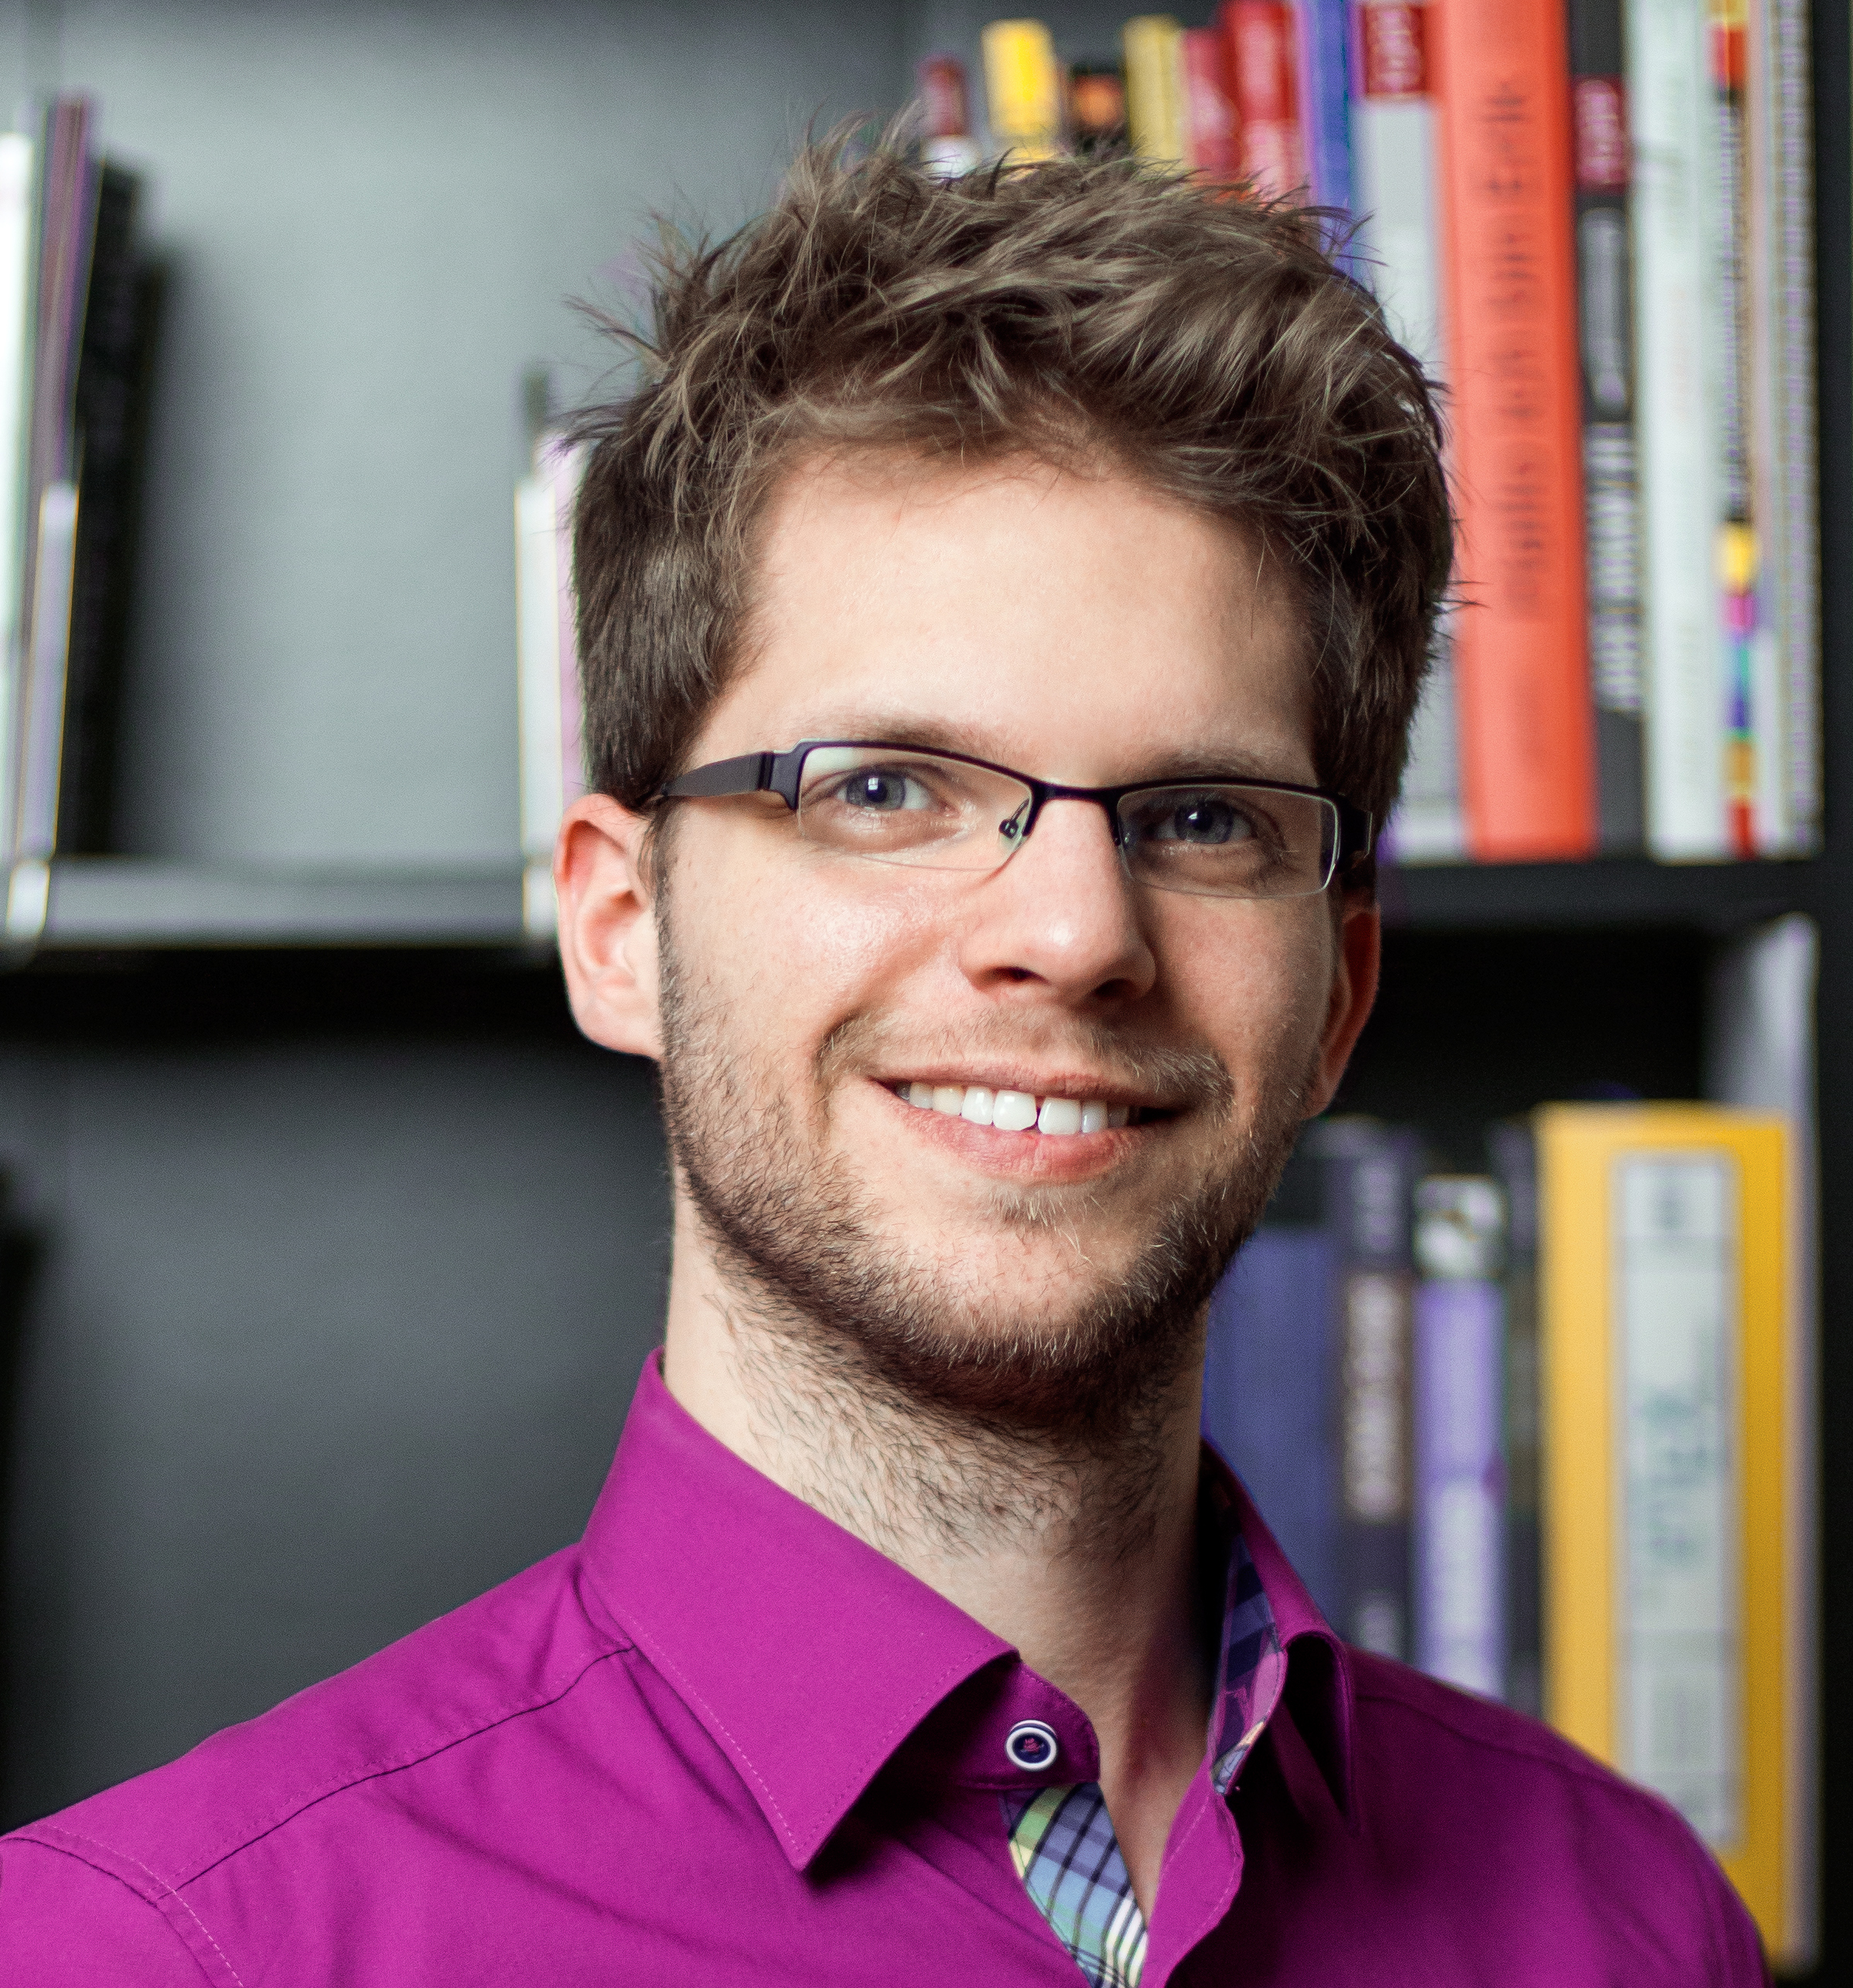
\includegraphics[width=\usedim{col-width}]{img/tobiw}
}

\setvar{logo}{%
   \TobiWLogo[width=40mm]
}

\setvar{timeline-birth}{1988}
\setvar{timeline-start}{2007}
\setvar{timeline-end}{2015}

\MakeCV

\end{document}